\documentclass{article}
\usepackage[utf8]{inputenc}
\usepackage{subfig}

%References
\usepackage{natbib}
%IMPORTANT use https://www.citationmachine.net/ if you need to generate references!
% \citep{reference} creates Harvard Style references throughout

%Colors
\usepackage{xcolor}

\usepackage[protrusion=true,expansion]{microtype}

%Code Markup
\usepackage[outputdir=cache]{minted}
%Syntax Highlighting Style
\definecolor{bggray}{RGB}{40,40,40}
\newmintedfile[javacode]{java}{
	style=fruity,
	bgcolor=bggray,
	linenos,
	breaklines,
	tabsize=2,
	obeytabs
}

\newmintedfile[bashoutput]{text} {
	style=fruity,
	bgcolor=bggray,
	breaklines,
	tabsize =2,
	obeytabs
}

\newmintedfile[armfile]{ARM} {
	style=fruity,
	bgcolor=bggray,
	breaklines,
	tabsize =2,
	obeytabs
}

%Page Margins and stuff
\usepackage{geometry}
 \geometry{
 a4paper,
 total={170mm,257mm},
 left=20mm,
 }

%Pictures
\usepackage{graphicx}
\graphicspath{ {./images/} }

%Move the title position
\usepackage{titling}

\setlength{\droptitle}{-8.5em} %Up, near the top but not too high

\title{Assignment 3 - CT2109 Object Oriented Programming: Data Structures and Algorithms}
\author{Daniel Hannon (19484286)}
\date{March 2021}

\begin{document}
	\maketitle
	%Sets to Harvard Style and links the references file
	\section{Problem Analysis}
	\subsection{Overview}
	\textit{For this assignment, you are going to write an application which tests if a sequence of numbers is a palindrome or not. Specifically, you are going to write fourdifferent methods(with meaningful names)which take a String as a parameter and returns a Boolean which represents whether or not the String is a pallindrome}

	\subsection{The Four different methods}
	\begin{itemize}
		\item \textbf{Method1:} Reverse all characters in a string and then compare the string to the original and determine if it's a pallindrome
		\item \textbf{Method2:} We compare every element on an element by element basis using a loop, first to the last, second to the second last and so on. If at any point two do not match it returns false immediately
		\item \textbf{Method3:} We are going to use ArrayStack and ArrayQueue to compare strings to see if they are valid or not
		\item \textbf{Method4:} We recursively reverse the string and then compare it
	\end{itemize}

	\subsection{Algorithm analysis}
	For method1 I figured availing of the String.substring() method would work and encapsulating it in a for loop\\
	Method 2 required the use of two indexes and would run so long as the rightmost index was larger the leftmost index, as any checks of the other way would be redundant.\\
	Method 3: required me to splice the string and store the values in a stack and a queue then pulling them, this required use of the String.charAt() method.\\
	Method 4: required the use of recursive string splicing, I did this by taking the first character of the string out and adding it to the end of the result of the method called with that character spliced out.\\
	\subsection{Pre Calculation analysis}
	I reckon that Method 2 would be fastest as its worst case is if the value given is a pallindrome so it would often not even complete two cycles in the while loop.
	\subsection{Graphing}
	In order to get an accurate graph(As shown below), I generated random binary strings of n size in increments of five and then plotted them in matlab the worst amount of operations was seemingly 4n and the best was very small.
	\section{Code}
	\javacode{Main.java}
	\newpage
	\section{Outputs}
		\begin{figure}[h!]
			\centering
			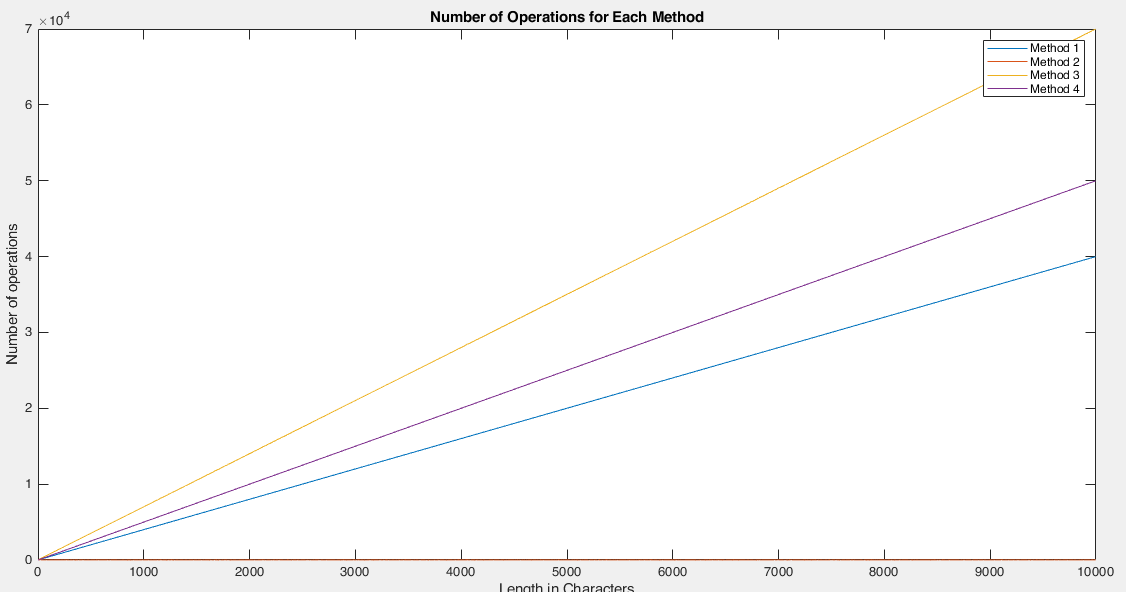
\includegraphics[width=\textwidth]{1.png}
			\caption{The four methods graphed by number of operations}
		\end{figure}
		\begin{figure}
			\centering
			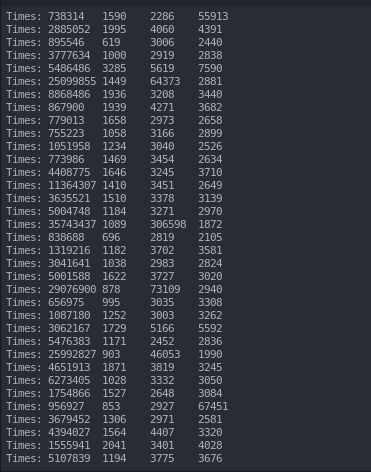
\includegraphics{2.png}
			\caption{A sample of the execution times for each method}
		\end{figure}
		\begin{figure}
			\centering
			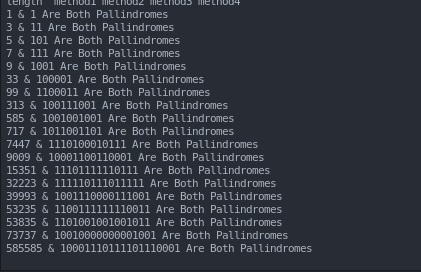
\includegraphics{3.png}
			\caption{List of dual pallindromes}
		\end{figure}
	\bibliographystyle{agsm}
	\bibliography{references}
\end{document}
